\subsection{Tranzitivní uzávěr}

\begin{definice}
  \textbf{Tranzitivní uzávěr} orientovaného grafu je orientovaný graf s
  původními vrcholy a platí, že existuje hrana z uzlu \emph{u} do uzlu \emph{v}
  právě tehdy, když v původním orientovaném grafu existuje libovolná orientovaná
  cesta z uzlu \emph{u} do uzlu \emph{v}.
\end{definice}

\begin{figure}[!ht]
  \begin{center}
    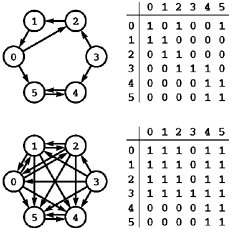
\includegraphics[scale=.7]{informatika/teoreticka_informatika/obrazky/tranzuzaver.png}
    \caption{Tranzitivní uzávěr grafu (zdroj: http://zorro.fme.vutbr.cz/graphs/foil36.html)}
  \end{center}
\end{figure}

\begin{poznamka}
  Platí, že matice dosažitelnosti v grafu $G$ = matice sousednosti tranzitivního
  uzávěru grafu $G$.
\end{poznamka}

\begin{obecne}{Algoritmus}
Z každého vrcholu vypustit DFS (Depth-first search~-- prohledávání do hloubky), do společné matice zaznamenávat dosažené vrcholy (řádek odpovídá vrcholu, sloupce vrcholům, které jsou z něho dosažitelné) -- složitost $O(n(n+m))$.
\end{obecne}

\begin{obecne}{Warshallův algoritmus}
Iterativní konstrukce matice dosažitelnosti, postupně počítá matice $W_k$, kde $w^{[k]}_{i, j} = 1$, pokud mezi vrcholy $i$ a $j$ existuje cesta, jejíž všechny vnitřní vrcholy jsou mezi vrcholy $1\dots k$.

Z matice $W_k$ lze spočítat matici $W^{[k+1]}: W^{[k+1]}_{i,j} = W^{[k]}_{i,j}  || (W^{[k]}_{i,k+1} \&\& W^{[k]}_{k+1,j})$ -- buď vede mezi vrcholy $i, j$ cesta, která nepoužije vrchol $k+1$, nebo taková, která ho použije -- v tom případě ale musí vést cesty mezi vrcholy $i,k+1$ a $k+1,j$, které používají pouze vrcholy $1\dots k$, jejich spojením je cesta mezi vrcholy $i,j$

Matice $W^1$ je matice incidence původního grafu.

Pseudokód (vstup: I -- matice incidence, $[0,1]^{n\times n}$):
\begin{verbatim}
Procedure Warshall(I)
W:= I;
for k:=1 to n
begin
  for i:=1 to n
  begin
    for j:=1 to n
\end{verbatim}
      $w_{i,j} = w_{i,j} || (w_{i,k} \&\& w_{k,j})$
\begin{verbatim}
  end
end 
return W;
\end{verbatim}

Složitost algoritmu je jasně $O(n^3)$ (potřebuje $2n^3$ bitových operací), což může být lepší pro grafy s hodně hranami (počet hran se blíží $n^2$), než složitost $n*DFS$ ( $n*(n + m) ≈ n * (n + n^2) = n^2 + n^3$ )

\end{obecne}

TODO: ještě něco?
